% !TeX root = Ausarbeitung_Anna-Lena_Marx.tex

\section{Einleitung}
Künstliche Intelligenz und maschinelles Lernen liegen in der Informatik momentan sehr im Trend, wie ein Blick auf den \textit{Gartner Hype Cycle} vom Juli 2017 \ref{pic:gartner} \cite{gartner} zeigt. Neben der Anwendung von künstlicher Intelligenz z.B. in virtuellen Assistenten oder autonomer Fahrzeuge, ist auch das Gebiet des maschinellen Lernens allgemein, aber auch im Speziellen mit Deep Learning und Deep Reinforcement Learning vertreten. Zwar befinden sich Deep Learning, Deep Reinforcement Learning und Machine Learning laut dieser Grafik mit Stand 2017 noch in einer relativ frühen Phase, aber es ist zu erwarten, dass beide Technologien die Industrie in absehbarer Zeit in der Breite erreichen. Laut der Abbildung dürfte Deep Learning erst in den nächsten Jahren tatsächlich produktiv in der Industrie zu finden sein, aber das Interesse dieser scheint groß zu sein. 
Die Idee hinter Deep Learning, beziehungsweise künstlichen neuronalen Netzen, existiert in der Informatik schon seit den 1940er Jahren \cite{Kriesel2007NeuralNetworks} doch erst mit der Rechenleistung heutiger Computer kann sich diese auch außerhalb der Forschung durchsetzen. 
Damit wächst allerdings auch der Bedarf der Industrie an Experten schneller an der Lehrplan der Hochschulen daran angepasst werden kann und auch in anderen Fachgebieten wird immer mehr ein gewisses Grundwissen erwartet um eine reibungslose Zusammenarbeit zwischen den Disziplinen zu erreichen. \\
\\
Mit der Lehrveranstaltung \textit{Künstliche Intelligenz} der Hochschule Pforzheim wurde eine solche Grundlage geschaffen. Die vorliegende Arbeit dokumentiert die exemplarische Anwendung der erlernten theoretischen Grundlagen im Bereich des Deep Learnings. Im folgenden soll mit Hilfe des Frameworks \textit{Keras} ein neuronales Netz erstellt und anhand des belgischen Verkehrszeichen Datensatzes trainiert und evaluiert werden. 

\begin{figure} [H]
	\centering
	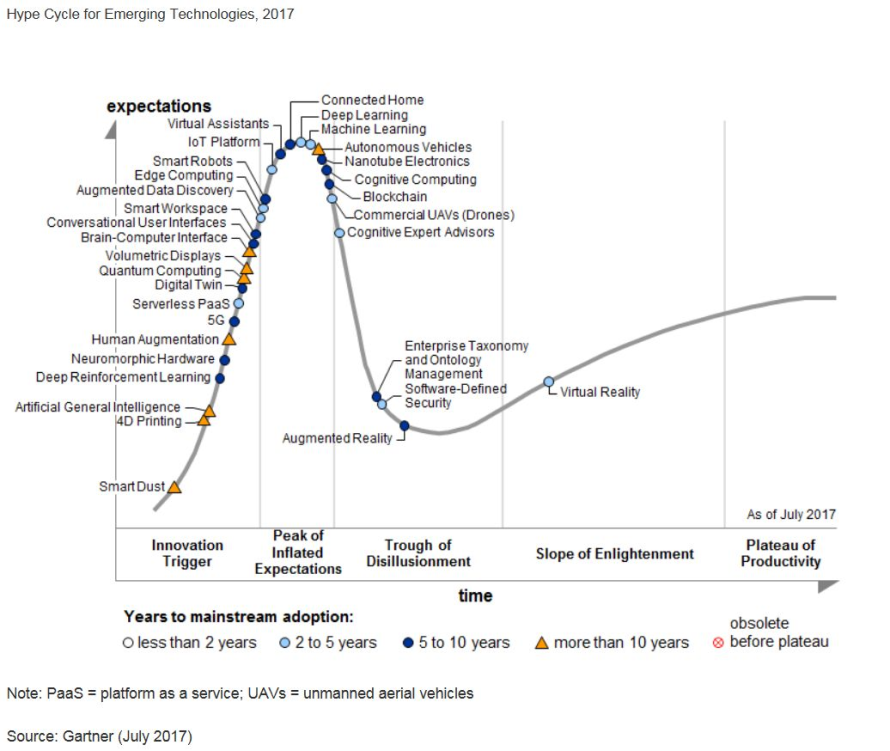
\includegraphics[scale=0.35]{gartner}
	\caption{Gartner Hype Cycle 2017 \cite{gartner}}
	\label{pic:gartner}
\end{figure}

%TODO verweis auf angehängte Dateien/Github
\subsection{Quellcodes}
Alle Dateien und Quellcodes, die notwendig sind, um diese Arbeit nachzuvollziehen sind im GitHub Repository \url{https://github.com/Allegra42/ki-keras-belgian-traffic-sign} abgelegt. Die benötigten Abhängigkeiten können z.B. über \texttt{virtualenv} und den Befehl \texttt{pip install -r requirements.txt} installiert werden. Das Training der Modelle kann über den Befehl \texttt{python3\ Keras.py} gestartet werden. Dabei wird angenommen, dass die Trainings- und Testdaten bereits heruntergeladen und unter dem Pfad \texttt{/data/} entpackt sind. Ist dies nicht der Fall kann im Quellcode die Zeile 222, \texttt{download\_data()} in der Methode \texttt{setup\_data()}, einkommentiert werden. Um ein Modell auf beliebige, entsprechend der Bildausschnitte der Trainingsbilder zugeschnittene, Bilder anzuwenden, dient der Befehl \texttt{python3 ClassifyImages.py -m <Pfad/zum/Modell> -i <Pfad/zum/Bild>}. Alle Anwendungen, die im Rahmen dieser Arbeit erstellt wurden, sind nur auf Linux entwickelt und getestet worden. Bei einem Systemwechsel müssen die Pfadangaben in den Quellcodes und den Aufrufen der Anwendungen entsprechend angepasst werden. 
\newpage